\section{Basic Artificial Neural Network}
Artificial neural networks (ANNs) are biologically inspired computer programs designed to simulate the way in which the human brain processes information.
%This model is just a model for a class of parameterized function with some special function structure which can be presented simply using some simple network graph. This method is began from the approximation of neural network in human.
\subsection{basic element: Nonlinear active function with affine map}
Mc Culloch-Pitts Neuron, also known as M-P Neuron, is the earliest neural network that was discovered in 1943. In this model, the neurons are connected by connection weights, and the activation function is used in binary. The threshold is used to determine whether the neuron will fire or not.

M-P element(approximation of one neuron): this is a very simple example for interpolating a function $f: \mathbb{R}^m \to \mathbb{R}$, with the next definition:
\begin{equation}\label{eq:M-P}
f_{M-P}(x) = \sigma( w \cdot x + b)
\end{equation}
with $w  \in \mathbb{R}^{m} $ and $\sigma$ is called active function which can be chosen like:
\begin{equation}
\sigma (x) = \frac{1}{1 + e^{-x}},
\end{equation}
or
\begin{equation}
\sigma(x) = tanh(x) = \frac{e^x - e^{-x}}{e^x + e^{-x}}.
\end{equation}
Basically, both these two functions are smooth and have two horizontal asymptotic lines, which can be seen as a smoothing approximation for
\begin{equation}
H(x) =
\begin{cases}
1  &\text{if}  ~x < 0, \\
0 &\text{if}~ x \le 0.
\end{cases}
\end{equation}
But now, the most commonly used activation function is the so-called ``Rectified Linear Unit'' (ReLU), which is defined by
\begin{equation}
{\rm ReLU}(x) = \max\{0,x\}.
\end{equation}
%We will talk about some basic stuff about variant of activation function in the next chapter and 
It is also very important in the approximation theory for such as one hidden layer ANN networks.
This is often shown as the next picture:
\begin{figure}[!ht]
	\center{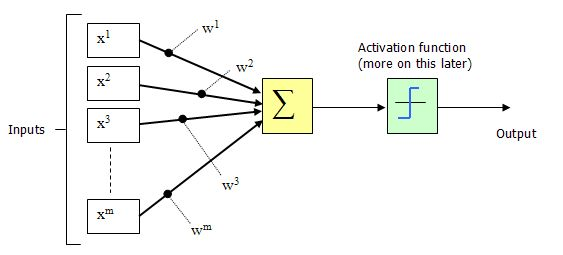
\includegraphics[width=10cm] {M-P.jpeg}}
	\caption{M-P neuron.}
\end{figure}

\subsection{neural network}
Now we want to use this simple basic element to construct some more complex model(from one neuron to neural network). A bionic but simple construction is to increase the basic element in both horizontal and vertical direction, which means the network would be like the one in Fig~\ref{fig:ANN}.
\begin{figure}[!ht]
	\center{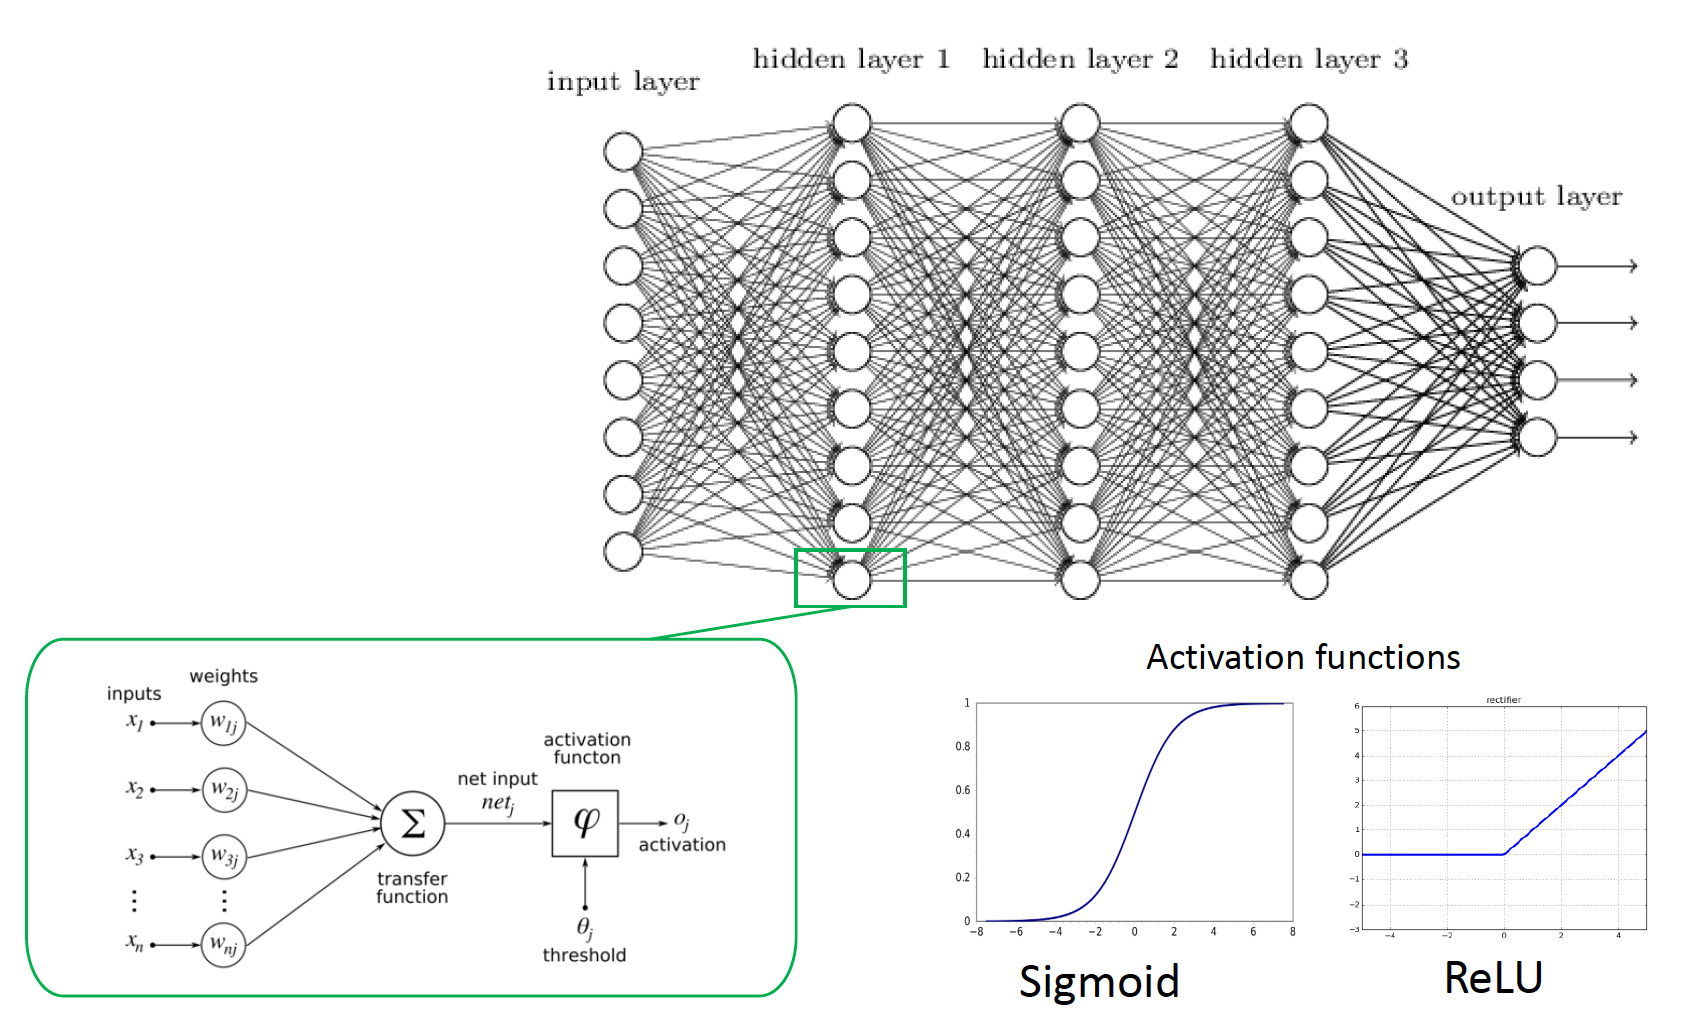
\includegraphics[width=12cm,height=6cm] {ANN.png}}
	\caption{ANN}
	\label{fig:ANN}
\end{figure}

This is called fully connected feedforward neural network. Now we want to give a more compressive expression, we collect all the output in $k$-th level $[f^{k}]_l$, $l = 1,\cdots, n_k$.
So we can have the output in $k+1$-th level under this setting with
\begin{equation}
{f}^{k+1} = \theta^{k+1}\circ \sigma (f^{k})
\end{equation}
with
\begin{equation}
\theta^k(x) = w^kx+b \in\mathbb{R}^{n_{k+1}},
\end{equation} 
where 
\begin{equation}
w^k= 
\begin{pmatrix}
w_1 \\
\vdots \\
w_{n_{k+1}}
\end{pmatrix},\qquad \mbox{ with }\qquad w_i \in \mathbb{R}^{n_k}.
\end{equation} 

So, we get the final iterative definition with the last output and initial input of this network like:
\begin{equation}
\begin{cases}
f^{0} &= \theta^0(x), \\
f^{\ell} &= \theta^{\ell}\circ \sigma(f^{\ell-1}), \quad \ell = 1:J, \\
f(x;\Theta) &= f^J.
\end{cases}
\end{equation}
Here we note 
\begin{equation}
\Theta = \{ (\theta^0, \cdots, \theta^J) \}.
\end{equation}

%\subsection{Interpolation by optimization}
%So the  interpolation process can be seen as a optimization problem in the special function class if the activation function for every elements and  the network structure parameter $\mathcal{N}_K$ are given:
%\begin{equation}
%\mathcal{F} = \{\bm{f}_K(W_K;\bm{x}) ~|~  \bm{f}_0 = (\bm{x}^{T},1)^{T}\},
%\end{equation}
%and the optimization problem can be seen as
%\begin{equation}
%%\mathop{\min}_{f \in \mathcal{F}}  \frac{1}{N}\sum_{i=1}^N \|f(X^i) - Y^i\|^2 =
%\mathop{\min}_{W_K \in T_3(\mathcal{N}_K)}  L(W_K) := \frac{1}{N}\sum_{i=1}^N \|\bm{f}_K(W_K; X^i) - Y^i\|^2.
%\end{equation}
%But $\mathcal{F}$ this is neither a linear space nor a convex set.

%\iffalse
\subsection{Back-Propagation}
Here we will talk about how to compute $\nabla_{\Theta} f(x;\Theta)$ by using chain rule which is called Back-Propagation (BP) algorithm in deep learning. 
Thus we have
\begin{equation}
\frac{\partial {f}(x; \Theta)}{ \partial w^k} = \frac{\partial {f}^J}{\partial {f}^{J-1}} \cdot \frac{ \partial {f}^{J-1}}{\partial {f}^{J-2}} \cdots \frac{ \partial {f}^k}{\partial w^k}.
\end{equation}
We can see from the above that, we only need to compute those terms like:
\begin{equation}
\frac{ \partial {f}^k}{\partial w^{k}}  \quad \text{and} \quad \frac{\partial {f}^k}{\partial {f}^{k-1}}  \quad k = 1,2,\cdots,J.
\end{equation}
We have
\begin{equation}\label{eq:partial-f}
\frac{\partial {f}^k}{\partial {f}^{k-1}} =
w^k{\rm Diag}(\sigma'(f^{k-1})) ,
\end{equation}
and
\begin{equation}
\frac{ \partial {f}^k}{\partial w^{k}}  = \delta \otimes \sigma(f^{k-1}).
\end{equation}


In short, BP algorithm can be expressed as:
\begin{algorithm}[H]
	\begin{algorithmic}[1]
		\State {\bf{Input:}}  $X^i$ and $W_K$;
		\For{$k = K:-1:1$}
		\State Compute and save
		$$\frac{ \partial {f}^k}{\partial w^{k}}  \quad \text{and} \quad \frac{\partial {f}^k}{\partial {f}^{k-1}}$$.
		\State Compute
		$$\frac{ \partial {f}^J}{\partial w^{k}} = \frac{\partial {f}^J}{\partial {f}^{J-1}} \cdot \frac{ \partial {f}^{J-1}}{\partial {f}^{J-2}} \cdots \frac{ \partial {f}^k}{\partial w^{k}}$$ 
		\EndFor
	\end{algorithmic}
	\caption{Back-Propagation Algorithm}
\end{algorithm}




%\subsection{Classical DNN}
First, we have a more comprehensive notation for classical DNN models.
\begin{equation}\label{eq:DNNdef_J}
\begin{aligned}
{\rm{DNN}_J} :=\{& f:f=
\theta^J \circ \sigma \circ \theta^{J-1} \cdots \sigma \circ \theta^0(x), \\
&\theta^\ell \in \mathbb{R}^{n^{\ell+1} \times (n^\ell+1)}, \quad n^0 = d, \quad n^{J+1} = 1, \quad n^\ell \in \mathbb{N}^+\}.
\end{aligned}
\end{equation}

Thus to say, we have the general two definition for DNN with
\begin{itemize}
\item  $\sigma \circ \theta$ type:
\begin{equation}\label{eq:sigma+theta}
\begin{aligned}
f^0 &= x, \\
f^{i+1} &= \sigma \circ \theta^{i}(f^i), \\
{\rm DNN}_J &= \{\theta^J(f^J)\}.
\end{aligned}
\end{equation}

\item $\theta \circ \sigma $ type:
\begin{equation}\label{eq:theta+sigma}
\begin{aligned}
f^0 &= \theta^0(x), \\
f^{i+1} &=  \theta^{i+1} \circ \sigma (f^i), \\
{\rm DNN}_J &= \{f^J\}.
\end{aligned}
\end{equation}
\end{itemize}

\subsection{DNN type ResNet}
For simplicity, we choose $\sigma \circ \theta$ type as example.

\paragraph{ResNet}
The ResNet can be written as
\begin{equation}\label{ori-ResNet-dnn}
\begin{cases}
f^0 &= x, \\
f^{i} &= \sigma \left( P^i f^{i-1} + \mathcal{F}^{ i} (f^{i-1}) \right), \quad i = 1:J ,\\
{\rm ResNet}_{J} &= \{  \theta^J f^{J} \}.
\end{cases}
\end{equation}
Here
\begin{equation}\label{eq:F-ResNet}
\mathcal{F}^{i} (f^{i-1}) = \xi^{i} \circ \sigma \circ \eta^{i} (f^{i-1}),
\end{equation}
means ResNet with skip connection distant 2. And $P^i$ is use to fit the dimension as
\begin{equation}\label{eq:P^i}
P^i: \mathbb{R}^{n_{i-1}} \mapsto \mathbb{R}^{n_i}.
\end{equation}

\paragraph{iResNet} 
The iResNet can be written as:
\begin{equation}\label{ori-iResNet-dnn}
\begin{cases}
f^0 &= x, \\
f^{i} &=  P^i f^{i-1} + \mathcal{F}^{ i} (f^{i-1}) , \quad i = 1:J ,\\
{\rm iResNet}_{J} &= \{  \theta^J f^{J} \}.
\end{cases}
\end{equation}
Here
\begin{equation}\label{eq:F-iResNet}
\mathcal{F}^{i} (f^{i-1}) = \xi^{i} \circ \sigma \circ \eta^{i}  \circ \sigma (f^{i-1}),
\end{equation}
means iResNet with skip connection distant 2. 
And $P^i$ is use to fit the dimension as in ResNet in \eqref{eq:P^i}.

The only difference between ResNet and iResNet can be viewed as 
putting a $\sigma$ in different places. 

And we also need to notice that ${\rm ResNet}_J$ or  ${\rm iResNet}_J$
are often called DNN with $2J$-th layers if the distance of skip connection
is $2$ as in \eqref{eq:F-ResNet} and \eqref{eq:F-iResNet}.

\subsection{DNN type MgNet}
Similar with ResNet, we can rewrite MgNet.

Here use $\theta \circ \sigma$ type as example.
\begin{equation}\label{ori-MgNetNet-dnn}
\begin{cases}
f^0 &= 0, \quad f^0 = \theta^0(x) \\
f^{i} &=  P^i f^{i-1} + \mathcal{F}^{ i} (f^{i-1}) , \quad i = 1:J ,\\
{\rm iResNet}_{J} &= \{  f^{J} \}.
\end{cases}
\end{equation}
Here
\begin{equation}\label{eq:F-MgNet}
\mathcal{F}^{i} (f^{i-1}) = \xi^{i} \left( f^{i-1} +  \sigma \circ \eta^{i} \circ \sigma(f^{i-1}) \right).
\end{equation}

\subsection{DNN type DenseNet}
In fact, DenseNet might be simple for definition in DNN case. 

Here use $\sigma \circ \theta$ type as example.
\begin{equation}\label{ori-DenseNet-dnn}
\begin{cases}
f^0 &= x, \\
f^{i} &=   \sigma \circ \theta^{i}([f^{i-1}, f^{i-2}, \cdots, f^0]) , \quad i = 1:J ,\\
{\rm DenseNet}_{J} &= \{  \theta^J f^{J} \}.
\end{cases}
\end{equation}

Here $[f^{i-1}, f^{i-2}, \cdots, f^0]$ means a long vector by collecting all 
outputs from $f^0$ to $f^{i-1}$, thus to say
$$
{\rm dim}([f^{i-1}, f^{i-2}, \cdots, f^0]) = \sum_{i=0}^{i-1} n_i.
$$


\section{A Universal DNN Model}

\subsection{Kailai's definition}
A DNN is defined as a tuple $M=(\mathcal{S}, \mathcal{O}, s_0, F, \delta)$
\begin{itemize}
	\item $\mathcal{S}$ is a non-empty set of states.
	\item $\mathcal{O}$ is a finite, non-empty set of parametrized operators.
	\item $s_0\in \mathcal{S}$ is the initial input. 
	\item $F\subset \mathcal{S}$ is the set of final states~(outputs). 
	\item $\delta: 2^{\mathcal{S}}\times \mathcal{O} \rightarrow \mathcal{S}$ is the mapping function. 
\end{itemize}
and an acceptable ordered sequence $(\delta_1, \delta_2, \ldots, \delta_n)$, which maps $s_0$ to $\delta_n \circ \delta_{n-1} \circ \delta_1 (s_0) \in F$.

\subsection{Juncai's definition}
The idea is that, deep neural network comes from the composition of linear and 
element-wise activation. 
So, we define the basic component of our model as:
\begin{equation}
\mathcal L_{\sigma,1}(x) = Wx + b + \sigma(\tilde Wx + \tilde b),
\end{equation}
where 
\begin{equation}
x \in \mathbb{R}^d, \quad W, ~ \tilde W \in \mathbb{R}^{n \times d} \quad \text{and} \quad b,~ \tilde b \in \mathbb{R}^n.
\end{equation}
Then we try to define an important operator in the universal DNN model,
known as $\mathcal L_{\sigma, \ell}(x^1, \cdots, x^k)$, by recursion of $\mathcal L_{\sigma,1}$. 
For $x^i \in \mathbb{R}^{n_i}, i = 1:\ell$,  we have
\begin{equation}
\mathcal L_{\sigma, \ell}(x^1, \cdots, x^k) = \mathcal L_{\sigma,1}
\left([\mathcal L_{\sigma, \ell-1}(\hat x^1), \mathcal L_{\sigma, \ell-1}(\hat x^2), \cdots, \mathcal L_{\sigma, \ell-1}(\hat x^k)]\right),
\end{equation}
where
\begin{equation}
\mathcal L_{\sigma, \ell-1}(\hat x^k) = \mathcal L_{\sigma, \ell-1} (x^1, \cdots, x^{k-1}, x^{k+1}, \cdots, x^\ell),
\end{equation}
and 
\begin{equation}
[\mathcal L_{\sigma, \ell-1}(\hat x^1), \mathcal L_{\sigma, \ell-1}(\hat x^2), \cdots, \mathcal L_{\sigma, \ell-1}(\hat x^k)],
\end{equation}
means to collect all the output of $\mathcal L_{\sigma, \ell-1}(\hat x^k)$ into one vector such 
that it can be the input of $\mathcal L_{\sigma, 1}$.

Then we define the $J-$layer universal DNN model by recursion as:
\begin{equation}
\begin{cases}
f^{0} &= x,  \\
f^{\ell} &= \mathcal L_{\sigma, \ell}(f^0,\cdots, f^{\ell-1}), \quad \ell = 1:J, \\
f(x) &= W^J f^J + b^J. 
\end{cases}
\end{equation}




